\documentclass[12pt]{article}\usepackage[]{graphicx}\usepackage[]{color}
% maxwidth is the original width if it is less than linewidth
% otherwise use linewidth (to make sure the graphics do not exceed the margin)
\makeatletter
\def\maxwidth{ %
  \ifdim\Gin@nat@width>\linewidth
    \linewidth
  \else
    \Gin@nat@width
  \fi
}
\makeatother

\definecolor{fgcolor}{rgb}{0.345, 0.345, 0.345}
\newcommand{\hlnum}[1]{\textcolor[rgb]{0.686,0.059,0.569}{#1}}%
\newcommand{\hlstr}[1]{\textcolor[rgb]{0.192,0.494,0.8}{#1}}%
\newcommand{\hlcom}[1]{\textcolor[rgb]{0.678,0.584,0.686}{\textit{#1}}}%
\newcommand{\hlopt}[1]{\textcolor[rgb]{0,0,0}{#1}}%
\newcommand{\hlstd}[1]{\textcolor[rgb]{0.345,0.345,0.345}{#1}}%
\newcommand{\hlkwa}[1]{\textcolor[rgb]{0.161,0.373,0.58}{\textbf{#1}}}%
\newcommand{\hlkwb}[1]{\textcolor[rgb]{0.69,0.353,0.396}{#1}}%
\newcommand{\hlkwc}[1]{\textcolor[rgb]{0.333,0.667,0.333}{#1}}%
\newcommand{\hlkwd}[1]{\textcolor[rgb]{0.737,0.353,0.396}{\textbf{#1}}}%
\let\hlipl\hlkwb

\usepackage{framed}
\makeatletter
\newenvironment{kframe}{%
 \def\at@end@of@kframe{}%
 \ifinner\ifhmode%
  \def\at@end@of@kframe{\end{minipage}}%
  \begin{minipage}{\columnwidth}%
 \fi\fi%
 \def\FrameCommand##1{\hskip\@totalleftmargin \hskip-\fboxsep
 \colorbox{shadecolor}{##1}\hskip-\fboxsep
     % There is no \\@totalrightmargin, so:
     \hskip-\linewidth \hskip-\@totalleftmargin \hskip\columnwidth}%
 \MakeFramed {\advance\hsize-\width
   \@totalleftmargin\z@ \linewidth\hsize
   \@setminipage}}%
 {\par\unskip\endMakeFramed%
 \at@end@of@kframe}
\makeatother

\definecolor{shadecolor}{rgb}{.97, .97, .97}
\definecolor{messagecolor}{rgb}{0, 0, 0}
\definecolor{warningcolor}{rgb}{1, 0, 1}
\definecolor{errorcolor}{rgb}{1, 0, 0}
\newenvironment{knitrout}{}{} % an empty environment to be redefined in TeX

\usepackage{alltt}

%\usepackage[roman]{../pres1}
%\usepackage[sans]{../pres1}

\usepackage[hmargin=1in,vmargin=1in]{geometry}
\usepackage{parskip}
\usepackage{hyperref}
\usepackage{graphicx}
\hypersetup{pdfstartview=FitV,hidelinks}





\IfFileExists{upquote.sty}{\usepackage{upquote}}{}
\begin{document}

{
  \Large
  \centering
  Lab 8 Assignment --- Metapopulation Models \\
  Due before Monday \\
}

\vspace{6pt}

Answer each of the following questions and upload your Excel file and
R script to ELC. Be sure to show your calculations. Undergraduates
only have to do Exercise I in R. \\
% Name the 
% file something like: \texttt{Chandler\_Richard-lab7.xlsx}. \\

\vspace{6pt}

\section*{Exercise I: Occupancy-based metapopulation models}


Imagine a metapopulation consisting of 16 sites. In the first year
($t=0$), the first 2 sites are occupied and the other 14 are not.
\begin{enumerate}
  \item[(a)] Project the metapopulation forward 40 years using a
    stochastic non-spatial model with colonization ($\gamma$) equal to
    0.3 and local extinction ($\epsilon$) equal to 0.2.

    Hint: to simulate whether a site is occupied or not in a given year,
    you must first compute occupancy probability ($\psi$) and then generate
    the binary presence/absence value using a Bernoulli distribution. The
    best way to generate a Bernoulli random variable in Excel is to use
    the \texttt{IF} and \texttt{RAND} functions, not the Bernoulli
    random number generator. Your formula should look something like
    \texttt{=IF(RAND()<\textcolor{blue}{CELL}, 1, 0)} with \texttt{\textcolor{blue}{CELL}} replaced by an
    actual cell containing the expected occurrence probability
    ($\psi$). It will be much faster to drag these equations across
    cells for all years and sites, than it would be using the
    Bernoulli random number generator.

    Additional information: In short, the \texttt{RAND} function draws a
    random number between 0 and 1. The \texttt{IF} function returns a 1 if
    this value is less than occupancy probability ($\psi$), or it returns
    a 0 if the random number is greater than $\psi$. This is doing the
    same thing as using the Bernoulli distribution to draw a random
    number.
  \item[(b)] Make a graph of the proportion of sites occupied (PrO)
    on the y-axis, and time on the x-axis.
  \item[(c)] According to this model, is it possible for this
    metapopulation to go permanently extinct? Why or why not?
  \item[(d)] Repeat the simulation several times by double-clicking in
    an empty cell or hitting F9. Why does the metapopulation appear to
    converge to a stochastic equilibrium?
\end{enumerate}




\clearpage


\section*{Exercise II: Abundance-based metapopulation models }
You have been hired by the Charles Darwin Research Center on the
Galapagos Islands. Your job is to assess a metapopulation of a species
of special concern -- the Magnificent Frigatebird.

\begin{figure}[h!]
  \centering
  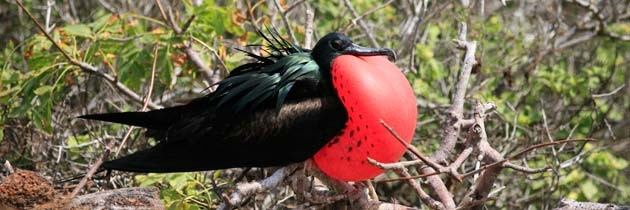
\includegraphics[width=\textwidth]{figs/frigatebird}
  \label{fig:frig}
\end{figure}

\vspace{-24pt}

% \subsection*{Part A}
% \vspace{-6pt}
Historical (fake) data showed that 2 populations of frigatebirds were
isolated for 40 years.

\begin{enumerate}
  \item[(a)] Project each population forward 40 years using the basic
    geometric growth model with $\lambda_1=1.05$ and
    $\lambda_2=0.95$. Calculate the final growth rate ($N_{t+1}/N_t$)
    for each population.
  \item[(b)] Next, imagine the 2 populations were actually connected
    in a small metapopulation. Use the abundance-based metapopulation
    model (including immigration and emigration) to project these
    connected subpopulations forward 40 years. Calculate the final
    growth rates for each population.
  \item[(c)] Make a graph of abundance vs. time for the isolated and
    connected populations.
  \item[(d)] Is site 2 a source or a sink? With this in mind,
    briefly describe the patterns you see in the graph and discuss the
    effects (positive and negative) of linking the two populations via
    dispersal if your goal was to sustain frigatebirds.
\end{enumerate}

% \subsection*{Part B}
% \vspace{-6pt}
% After further research, you have discovered that the frigatebirds
% currently occupy a metapopulation consisting of 4 subpopulations
% (islands). Movement probabilities and starting population sizes of
% subpopulations are given for you in Excel.

% \begin{enumerate}
%   \item[(a)] Using the abundance-based metapopulation model, project
%     the metapopulation forward 50 years. (Be especially careful about
%     locking cells and using the movement rates in the appropriate
%     places in the model).
%   \item[(b)] Create two graphs depicting population sizes ($n_{i,t}$)
%     and growth rates ($\lambda_{i,t}$) over time.
%   \item[(c)] Is this metapopulation viable or is it likely to go
%     extinct? Explain.
% \end{enumerate}




\clearpage


\section*{Occupancy based metapopulation models in {\tt R} }


Here is an example of how to simulate occupancy data. First, define
the parameters and create an empty matrix to store the binary
presence/absence data.

\begin{knitrout}
\definecolor{shadecolor}{rgb}{0.969, 0.969, 0.969}\color{fgcolor}\begin{kframe}
\begin{alltt}
\hlstd{nSites} \hlkwb{<-} \hlnum{10}
\hlstd{nYears} \hlkwb{<-} \hlnum{12}
\hlstd{gamma} \hlkwb{<-} \hlnum{0.2}    \hlcom{## Colonization probability}
\hlstd{epsilon} \hlkwb{<-} \hlnum{0.25} \hlcom{## Local extinction probability}
\end{alltt}
\end{kframe}
\end{knitrout}


Let's assume that we know that the first 8 sites were occupied in year
1. In practice, we would have to estimate initial occupancy.
\begin{knitrout}
\definecolor{shadecolor}{rgb}{0.969, 0.969, 0.969}\color{fgcolor}\begin{kframe}
\begin{alltt}
\hlstd{O} \hlkwb{<-} \hlstd{psi} \hlkwb{<-} \hlkwd{matrix}\hlstd{(}\hlnum{NA}\hlstd{, nYears, nSites)}
\hlstd{O[}\hlnum{1}\hlstd{,]} \hlkwb{<-} \hlkwd{c}\hlstd{(}\hlkwd{rep}\hlstd{(}\hlnum{1}\hlstd{,} \hlnum{8}\hlstd{),} \hlnum{0}\hlstd{,} \hlnum{0}\hlstd{)}
\end{alltt}
\end{kframe}
\end{knitrout}

In subsequent years, occupancy is determined by colonization and
extinction. We can simulate data using the {\tt rbinom}
function. When you set the {\tt size} argument to 1, {\tt rbinom}
generates random numbers from a Bernoulli distribution.
\begin{knitrout}
\definecolor{shadecolor}{rgb}{0.969, 0.969, 0.969}\color{fgcolor}\begin{kframe}
\begin{alltt}
\hlkwa{for}\hlstd{(t} \hlkwa{in} \hlnum{2}\hlopt{:}\hlstd{nYears) \{}
    \hlstd{psi.t} \hlkwb{<-} \hlstd{O[t}\hlopt{-}\hlnum{1}\hlstd{,]}\hlopt{*}\hlstd{(}\hlnum{1}\hlopt{-}\hlstd{epsilon)} \hlopt{+} \hlstd{(}\hlnum{1}\hlopt{-}\hlstd{O[t}\hlopt{-}\hlnum{1}\hlstd{,])}\hlopt{*}\hlstd{gamma}
    \hlstd{O[t,]} \hlkwb{<-} \hlkwd{rbinom}\hlstd{(nSites,} \hlkwc{size}\hlstd{=}\hlnum{1}\hlstd{,} \hlkwc{prob}\hlstd{=psi.t)}
\hlstd{\}}
\end{alltt}
\end{kframe}
\end{knitrout}

Take a look at the binary occupancy data.
\begin{knitrout}
\definecolor{shadecolor}{rgb}{0.969, 0.969, 0.969}\color{fgcolor}\begin{kframe}
\begin{alltt}
\hlstd{O}
\end{alltt}
\begin{verbatim}
##       [,1] [,2] [,3] [,4] [,5] [,6] [,7] [,8] [,9] [,10]
##  [1,]    1    1    1    1    1    1    1    1    0     0
##  [2,]    1    1    1    1    1    0    1    1    1     0
##  [3,]    0    1    1    0    1    0    0    0    0     0
##  [4,]    0    1    1    0    1    0    0    0    0     0
##  [5,]    0    1    1    0    1    1    0    0    0     0
##  [6,]    0    1    1    0    1    1    0    0    0     0
##  [7,]    0    1    1    0    1    1    0    1    0     0
##  [8,]    0    1    0    0    1    1    0    1    0     1
##  [9,]    0    1    0    0    1    0    0    0    0     1
## [10,]    0    1    0    0    1    0    0    0    0     1
## [11,]    0    1    0    1    1    1    1    1    0     1
## [12,]    0    1    0    1    1    0    1    0    0     0
\end{verbatim}
\end{kframe}
\end{knitrout}

Compute the number of sites occupied each year.
\begin{knitrout}
\definecolor{shadecolor}{rgb}{0.969, 0.969, 0.969}\color{fgcolor}\begin{kframe}
\begin{alltt}
\hlstd{nOccupied} \hlkwb{<-} \hlkwd{rowSums}\hlstd{(O)}
\hlstd{nOccupied}
\end{alltt}
\begin{verbatim}
##  [1] 8 8 3 3 4 4 5 5 3 3 7 4
\end{verbatim}
\end{kframe}
\end{knitrout}

\clearpage

Compute the proportion of sites occupied (PrO) each year.
\begin{knitrout}
\definecolor{shadecolor}{rgb}{0.969, 0.969, 0.969}\color{fgcolor}\begin{kframe}
\begin{alltt}
\hlstd{PrO} \hlkwb{<-} \hlstd{nOccupied} \hlopt{/} \hlstd{nSites}
\hlstd{PrO}
\end{alltt}
\begin{verbatim}
##  [1] 0.8 0.8 0.3 0.3 0.4 0.4 0.5 0.5 0.3 0.3 0.7 0.4
\end{verbatim}
\end{kframe}
\end{knitrout}

Graph it.
\begin{knitrout}
\definecolor{shadecolor}{rgb}{0.969, 0.969, 0.969}\color{fgcolor}\begin{kframe}
\begin{alltt}
\hlkwd{plot}\hlstd{(}\hlnum{1}\hlopt{:}\hlstd{nYears, PrO,} \hlkwc{type}\hlstd{=}\hlstr{"b"}\hlstd{,} \hlkwc{xlab}\hlstd{=}\hlstr{"Time"}\hlstd{,} \hlkwc{ylab}\hlstd{=}\hlstr{"Proportion of sites occupied"}\hlstd{,}
     \hlkwc{ylim}\hlstd{=}\hlkwd{c}\hlstd{(}\hlnum{0}\hlstd{,} \hlnum{1}\hlstd{))}
\end{alltt}
\end{kframe}
\includegraphics[width=\maxwidth]{figure/PrO-graph-1} 
\end{knitrout}


\clearpage

\section*{Abundance-based metapopulation models in \texttt{R}}

Suppose we have a metapopulation with 3 subpopulations characterized
by growth rates of $\lambda_1=0.98$, $\lambda_2=1$, and
$\lambda_3=1.02$. The transition probability matrix is:

\begin{table}[h!]
  \centering
  \begin{tabular}{ccc}
    \hline
    0.9 & 0.0 & 0.1 \\
    0.2 & 0.7 & 0.1 \\
    0.1 & 0.0 & 0.9 \\
    \hline
  \end{tabular}
\end{table}

Define parameters in \texttt{R}.
\begin{knitrout}
\definecolor{shadecolor}{rgb}{0.969, 0.969, 0.969}\color{fgcolor}\begin{kframe}
\begin{alltt}
\hlstd{lambda} \hlkwb{<-} \hlkwd{c}\hlstd{(}\hlnum{0.98}\hlstd{,} \hlnum{1}\hlstd{,} \hlnum{1.02}\hlstd{)}
\hlstd{pi} \hlkwb{<-} \hlkwd{matrix}\hlstd{(}\hlkwd{c}\hlstd{(}
    \hlnum{0.9}\hlstd{,} \hlnum{0.0}\hlstd{,} \hlnum{0.1}\hlstd{,}
    \hlnum{0.2}\hlstd{,} \hlnum{0.7}\hlstd{,} \hlnum{0.1}\hlstd{,}
    \hlnum{0.1}\hlstd{,} \hlnum{0.0}\hlstd{,} \hlnum{0.9}\hlstd{),} \hlkwc{nrow}\hlstd{=}\hlnum{3}\hlstd{,} \hlkwc{ncol}\hlstd{=}\hlnum{3}\hlstd{,} \hlkwc{byrow}\hlstd{=}\hlnum{TRUE}\hlstd{)}
\hlstd{nPatches} \hlkwb{<-} \hlnum{3}
\hlstd{nYears} \hlkwb{<-} \hlnum{50}
\end{alltt}
\end{kframe}
\end{knitrout}

Set the initial population sizes to 100, 110, and 120.
\begin{knitrout}
\definecolor{shadecolor}{rgb}{0.969, 0.969, 0.969}\color{fgcolor}\begin{kframe}
\begin{alltt}
\hlstd{n} \hlkwb{<-} \hlkwd{matrix}\hlstd{(}\hlnum{NA}\hlstd{, nYears, nPatches)}
\hlstd{n[}\hlnum{1}\hlstd{,]} \hlkwb{<-} \hlkwd{c}\hlstd{(}\hlnum{100}\hlstd{,} \hlnum{110}\hlstd{,} \hlnum{120}\hlstd{)}
\end{alltt}
\end{kframe}
\end{knitrout}

Project the metapopulation forward.
\begin{knitrout}
\definecolor{shadecolor}{rgb}{0.969, 0.969, 0.969}\color{fgcolor}\begin{kframe}
\begin{alltt}
\hlkwa{for}\hlstd{(t} \hlkwa{in} \hlnum{2}\hlopt{:}\hlstd{nYears) \{}
    \hlstd{n[t,}\hlnum{1}\hlstd{]} \hlkwb{<-} \hlstd{n[t}\hlopt{-}\hlnum{1}\hlstd{,}\hlnum{1}\hlstd{]}\hlopt{*}\hlstd{lambda[}\hlnum{1}\hlstd{]}\hlopt{*}\hlstd{(}\hlnum{1}\hlopt{-}\hlstd{pi[}\hlnum{1}\hlstd{,}\hlnum{2}\hlstd{]}\hlopt{-}\hlstd{pi[}\hlnum{1}\hlstd{,}\hlnum{3}\hlstd{])} \hlopt{+}
        \hlstd{n[t}\hlopt{-}\hlnum{1}\hlstd{,}\hlnum{2}\hlstd{]}\hlopt{*}\hlstd{lambda[}\hlnum{2}\hlstd{]}\hlopt{*}\hlstd{pi[}\hlnum{2}\hlstd{,}\hlnum{1}\hlstd{]} \hlopt{+} \hlstd{n[t}\hlopt{-}\hlnum{1}\hlstd{,}\hlnum{3}\hlstd{]}\hlopt{*}\hlstd{lambda[}\hlnum{3}\hlstd{]}\hlopt{*}\hlstd{pi[}\hlnum{3}\hlstd{,}\hlnum{1}\hlstd{]}
    \hlstd{n[t,}\hlnum{2}\hlstd{]} \hlkwb{<-} \hlstd{n[t}\hlopt{-}\hlnum{1}\hlstd{,}\hlnum{2}\hlstd{]}\hlopt{*}\hlstd{lambda[}\hlnum{2}\hlstd{]}\hlopt{*}\hlstd{(}\hlnum{1}\hlopt{-}\hlstd{pi[}\hlnum{2}\hlstd{,}\hlnum{1}\hlstd{]}\hlopt{-}\hlstd{pi[}\hlnum{2}\hlstd{,}\hlnum{3}\hlstd{])} \hlopt{+}
        \hlstd{n[t}\hlopt{-}\hlnum{1}\hlstd{,}\hlnum{1}\hlstd{]}\hlopt{*}\hlstd{lambda[}\hlnum{1}\hlstd{]}\hlopt{*}\hlstd{pi[}\hlnum{1}\hlstd{,}\hlnum{2}\hlstd{]} \hlopt{+} \hlstd{n[t}\hlopt{-}\hlnum{1}\hlstd{,}\hlnum{3}\hlstd{]}\hlopt{*}\hlstd{lambda[}\hlnum{3}\hlstd{]}\hlopt{*}\hlstd{pi[}\hlnum{3}\hlstd{,}\hlnum{2}\hlstd{]}
    \hlstd{n[t,}\hlnum{3}\hlstd{]} \hlkwb{<-} \hlstd{n[t}\hlopt{-}\hlnum{1}\hlstd{,}\hlnum{3}\hlstd{]}\hlopt{*}\hlstd{lambda[}\hlnum{3}\hlstd{]}\hlopt{*}\hlstd{(}\hlnum{1}\hlopt{-}\hlstd{pi[}\hlnum{3}\hlstd{,}\hlnum{1}\hlstd{]}\hlopt{-}\hlstd{pi[}\hlnum{3}\hlstd{,}\hlnum{2}\hlstd{])} \hlopt{+}
        \hlstd{n[t}\hlopt{-}\hlnum{1}\hlstd{,}\hlnum{1}\hlstd{]}\hlopt{*}\hlstd{lambda[}\hlnum{1}\hlstd{]}\hlopt{*}\hlstd{pi[}\hlnum{1}\hlstd{,}\hlnum{3}\hlstd{]} \hlopt{+} \hlstd{n[t}\hlopt{-}\hlnum{1}\hlstd{,}\hlnum{2}\hlstd{]}\hlopt{*}\hlstd{lambda[}\hlnum{2}\hlstd{]}\hlopt{*}\hlstd{pi[}\hlnum{2}\hlstd{,}\hlnum{3}\hlstd{]}
\hlstd{\}}
\end{alltt}
\end{kframe}
\end{knitrout}


Do the same projection, but use matrix multiplication.
\begin{knitrout}
\definecolor{shadecolor}{rgb}{0.969, 0.969, 0.969}\color{fgcolor}\begin{kframe}
\begin{alltt}
\hlkwa{for}\hlstd{(t} \hlkwa{in} \hlnum{2}\hlopt{:}\hlstd{nYears) \{}
    \hlstd{n[t,]} \hlkwb{<-} \hlkwd{t}\hlstd{(pi)} \hlopt \hlstd{(n[t}\hlopt{-}\hlnum{1}\hlstd{,]}\hlopt{*}\hlstd{lambda)}
    \hlcom{## Same as:}
    \hlcom{## n[t,] <- t(pi) %*% diag(lambda) %*% n[t-1,]}
\hlstd{\}}
\end{alltt}
\end{kframe}
\end{knitrout}


Calculate the growth rates.
\begin{knitrout}
\definecolor{shadecolor}{rgb}{0.969, 0.969, 0.969}\color{fgcolor}\begin{kframe}
\begin{alltt}
\hlstd{lambda.it} \hlkwb{<-} \hlstd{n[}\hlopt{-}\hlnum{1}\hlstd{,]} \hlopt{/} \hlstd{n[}\hlopt{-}\hlstd{nYears,]}
\hlcom{## Same as:}
\hlcom{## lambda.it <- n[2:nYears,] / n[1:(nYears-1),]}
\end{alltt}
\end{kframe}
\end{knitrout}


\clearpage

Visualize changes in abundance over time.
\begin{knitrout}
\definecolor{shadecolor}{rgb}{0.969, 0.969, 0.969}\color{fgcolor}\begin{kframe}
\begin{alltt}
\hlkwd{matplot}\hlstd{(n,} \hlkwc{type}\hlstd{=}\hlstr{"l"}\hlstd{,} \hlkwc{xlab}\hlstd{=}\hlstr{"Time"}\hlstd{,} \hlkwc{ylab}\hlstd{=}\hlstr{"Abundance"}\hlstd{,}
        \hlkwc{ylim}\hlstd{=}\hlkwd{c}\hlstd{(}\hlnum{0}\hlstd{,} \hlnum{220}\hlstd{),} \hlkwc{lwd}\hlstd{=}\hlnum{2}\hlstd{)}
\hlkwd{legend}\hlstd{(}\hlkwc{x}\hlstd{=}\hlnum{1}\hlstd{,} \hlkwc{y}\hlstd{=}\hlnum{220}\hlstd{,}
       \hlkwd{c}\hlstd{(}\hlstr{"Subpopulation 1"}\hlstd{,} \hlstr{"Subpopulation 2"}\hlstd{,} \hlstr{"Subpopulation 3"}\hlstd{),}
       \hlkwc{lty}\hlstd{=}\hlnum{1}\hlopt{:}\hlnum{3}\hlstd{,} \hlkwc{col}\hlstd{=}\hlnum{1}\hlopt{:}\hlnum{3}\hlstd{)}
\end{alltt}
\end{kframe}
\includegraphics[width=\maxwidth]{figure/Nmeta-plot-n-1} 
\end{knitrout}

\clearpage

Visualize changes in growth rates over time.
\begin{knitrout}
\definecolor{shadecolor}{rgb}{0.969, 0.969, 0.969}\color{fgcolor}\begin{kframe}
\begin{alltt}
\hlkwd{matplot}\hlstd{(lambda.it,} \hlkwc{type}\hlstd{=}\hlstr{"l"}\hlstd{,} \hlkwc{xlab}\hlstd{=}\hlstr{"Time"}\hlstd{,} \hlkwc{ylab}\hlstd{=}\hlstr{"Growth rate"}\hlstd{,}
        \hlkwc{ylim}\hlstd{=}\hlkwd{c}\hlstd{(}\hlnum{0.7}\hlstd{,} \hlnum{1.23}\hlstd{),} \hlkwc{lwd}\hlstd{=}\hlnum{2}\hlstd{)}
\hlkwd{legend}\hlstd{(}\hlkwc{x}\hlstd{=}\hlnum{5}\hlstd{,} \hlkwc{y}\hlstd{=}\hlnum{1.23}\hlstd{,}
       \hlkwd{c}\hlstd{(}\hlstr{"Subpopulation 1"}\hlstd{,} \hlstr{"Subpopulation 2"}\hlstd{,} \hlstr{"Subpopulation 3"}\hlstd{),}
       \hlkwc{lty}\hlstd{=}\hlnum{1}\hlopt{:}\hlnum{3}\hlstd{,} \hlkwc{col}\hlstd{=}\hlnum{1}\hlopt{:}\hlnum{3}\hlstd{)}
\hlkwd{abline}\hlstd{(}\hlkwc{h}\hlstd{=}\hlnum{1}\hlstd{,} \hlkwc{col}\hlstd{=}\hlstr{"grey"}\hlstd{,} \hlkwc{lty}\hlstd{=}\hlnum{1}\hlstd{)}
\end{alltt}
\end{kframe}
\includegraphics[width=\maxwidth]{figure/Nmeta-plot-lam-1} 
\end{knitrout}



\end{document}




